\documentclass[11pt]{article}
\usepackage[letterpaper,margin=1in]{geometry}
\usepackage[T1]{fontenc}
\usepackage{lmodern,microtype,amsmath,amssymb,amsthm,booktabs,graphicx,xcolor}
\usepackage{tcolorbox}
\tcbuselibrary{skins}
\usepackage[hidelinks]{hyperref}
\definecolor{routegreen}{HTML}{128675}
\definecolor{takeawayink}{HTML}{213337}
\newtcolorbox{takeaway}{
 enhanced,
 colback=routegreen!5!white,
 colframe=routegreen!5!white,
 colupper=takeawayink,
 boxrule=0pt,
 borderline west={2pt}{0pt}{routegreen},
 arc=2mm,
 boxsep=0pt,
 left=4mm,right=4mm,top=3mm,bottom=3mm,
 before skip=8pt,after skip=9pt,
 fontupper=\sffamily\small,
 before upper={\textcolor{routegreen}{\bfseries Takeaway}\par\smallskip}
}
\newtcolorbox{construction}{
 enhanced,
 title={Construction algorithm.},
 colback=takeawayink!3!white,
 colbacktitle=takeawayink,
 colframe=takeawayink,
 coltitle=white,
 colupper=takeawayink,
 boxrule=0pt,
 arc=2mm,
 boxsep=0pt,
 left=4mm,right=4mm,top=3mm,bottom=3mm,
 toptitle=2.5mm,bottomtitle=2.5mm,
 before skip=10pt,after skip=10pt,
 fonttitle=\sffamily\small\bfseries,
 fontupper=\ttfamily\small\raggedright
}
\newtheorem{theorem}{Theorem}
\newtheorem{proposition}[theorem]{Proposition}
\newtheorem{corollary}[theorem]{Corollary}
\newcommand{\R}{\mathbb R}
\graphicspath{{figures/}{graph_traversal/figures/}}
\renewcommand{\topfraction}{.9}
\renewcommand{\textfraction}{.08}
\renewcommand{\floatpagefraction}{.8}
\setlength{\textfloatsep}{12pt plus 2pt minus 2pt}
\setlength{\floatsep}{10pt plus 2pt minus 2pt}
\title{Minimum Separation and Locality\\in Geometric Graph Traversal}
\author{Jonathan R. Landers}
\date{November 22, 2026}
\makeatletter
\renewcommand{\@maketitle}{%
 \begin{center}
 {\LARGE\@title\par}\vskip .8em
 {\large\@author\par}\vskip .4em
 {\large\@date\par}
 \end{center}\par\vskip .8em
}
\makeatother

\begin{document}
\maketitle
\begin{abstract}
For vertices in $\R^d$ separated by at least $k>0$, with edges joining
endpoints at distance at most $R$, disjoint-ball packing gives
$\Delta\le(1+2R/k)^d-1$. The graph has $O(n(1+R/k)^d)$ edges and
$O(n(1+R/k)^{2d})$ graph triangles, subject to finite-$n$ caps.
At fixed dimension and $R/k$, these counts are linear: spatial hashing
constructs the radius graph in expected $O(n)$ time, breadth-first search
takes $O(n)$, and binary-heap Dijkstra takes $O(n\log n)$.
We specialize standard packing and graph algorithms to these assumptions,
with proofs, reproducible structural measurements, and a road example
showing how a straight-edge drawing preserves winding-road costs.
\end{abstract}

\section{The question and the model}
Minimum separation excludes triangle configurations with a side below
the cutoff. A local connection rule bounds the triangles whose three
edges are present, and hence the work of constructing and traversing the graph.

Let $P=\{p_1,\ldots,p_n\}\subset\R^d$, $n\ge1$, where $d\ge1$ is fixed.
We impose the minimum-separation promise
\begin{equation}\label{eq:sep}
 \|p_i-p_j\|_2\ge k>0\qquad(i\ne j).
\end{equation}
Let $G=(P,E)$ be a simple undirected graph satisfying
\begin{equation}\label{eq:local}
 \{p_i,p_j\}\in E\quad\Longrightarrow\quad \|p_i-p_j\|_2\le R,
 \qquad R\ge0.
\end{equation}
Edges may form any subset of the pairs within range. The \emph{full radius
graph} includes all such pairs. Write $m=|E|$, let $\Delta$ be the maximum
degree, and let $T$ count unordered graph triangles. Define the dimensionless
ratio $\rho=R/k$. Vertex positions may be irregular, and edges may cross.

If $R<k$, every vertex is isolated; a connected graph with $n>1$ therefore
requires $R\ge k$. Traversal applies to each reachable component.

\paragraph{What distances mean.}
Separation and locality concern \emph{Euclidean endpoint distance}; edge
costs may be any supplied finite nonnegative values, including road arc
length or travel time. Arc length is at least endpoint distance, so a
maximum arc length $R$ implies \eqref{eq:local}. Endpoint-local roads may
wind arbitrarily. We assume constant-time cost lookup and arithmetic;
extracting costs from detailed geometry is separate preprocessing.

\section{Separation and connectivity}
\begin{proposition}\label{prop:alone}
For every $n\ge1$ and $k>0$, there is a planar set of $n$ vertices with
pairwise separation at least $k$ whose complete graph has $\binom n2$
edges and $\binom n3$ graph triangles.
\end{proposition}
\begin{takeaway}
Separated vertices can all connect to one another, allowing every triple
to form a graph triangle.
\end{takeaway}

\begin{proof}
Place $n$ distinct points on a circle large enough to separate every pair
by at least $k$, then connect every pair. This gives the stated counts;
every triple is a nondegenerate Euclidean triangle satisfying the cutoff.
\end{proof}

Scaling a finite point set by $k/\delta$, where $\delta>0$ is its minimum
separation, preserves topology; uniformly scaling costs preserves optimal routes.

Fixed dimension matters: an arbitrary metric allows any number of points
at mutual distance $k$ inside a radius-$k$ ball. Other metrics require
a packing hypothesis.

The separated triangle $(0,0),(k,0),(2k,\varepsilon)$ has area tending to
zero; minimum-angle conditions add further structure.

\section{Packing converts separation into local density}
\begin{theorem}[Local occupancy]\label{thm:packing}
For any $x\in\R^d$ and $r\ge0$, the number of vertices in the closed ball
$B(x,r)$ satisfies
\begin{equation}\label{eq:occupancy}
 |P\cap B(x,r)|\le \left(1+\frac{2r}{k}\right)^d.
\end{equation}
\end{theorem}
\begin{takeaway}
Because each vertex needs its own space, only a limited number can fit
inside a neighborhood of fixed size.
\end{takeaway}

\begin{proof}
The open radius-$k/2$ balls centered at vertices of $P\cap B(x,r)$ are
disjoint by \eqref{eq:sep} and lie inside $B(x,r+k/2)$. With unit-ball
volume $v_d$ and $N=|P\cap B(x,r)|$, volume comparison gives
\[
 N v_d(k/2)^d\le v_d(r+k/2)^d.
\]
Cancel the common factors.
\end{proof}

\begin{corollary}[Degree, edges, and graph triangles]\label{cor:counts}
Set $D=\min\{n-1,\lfloor(1+2\rho)^d\rfloor-1\}$. Then
\begin{equation}\label{eq:counts}
 \Delta\le D,\qquad m\le\frac{nD}{2},\qquad
 T\le\frac n3\binom D2.
\end{equation}
In particular, in the plane,
\[
 m=O\!\left(n\min\{n,(1+\rho)^2\}\right),\qquad
 T=O\!\left(n\min\{n^2,(1+\rho)^4\}\right).
\]
\end{corollary}
\begin{takeaway}
When the dimension and the ratio $R/k$ stay fixed, each vertex has only a
bounded number of neighbors, so edges and graph triangles grow at most
linearly with the network size.
\end{takeaway}

\begin{proof}
Apply Theorem~\ref{thm:packing} to $B(p_i,R)$ and subtract its central
vertex to bound degree. The identity $2m=\sum_i\deg(p_i)$ bounds edges.
Counting each triangle at its three vertices gives
\[
 3T\le\sum_i\binom{\deg(p_i)}2\le n\binom D2.
\]
\end{proof}

\begin{figure}[!htbp]
\centering
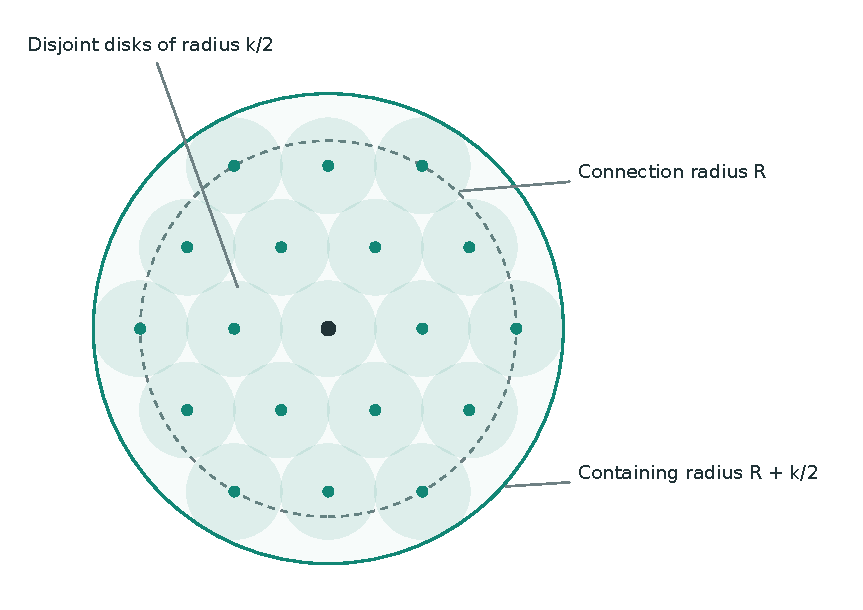
\includegraphics[width=.65\linewidth]{packing_bound.pdf}
\caption{The planar packing argument, illustrated at $R=2k$. Disks of
radius $k/2$ around a vertex and its possible neighbors have disjoint
interiors and fit in a disk of radius $R+k/2$. The outer boundary
contains all the packing disks.}
\label{fig:packing}
\end{figure}

Fixed $d$ and bounded $\rho$ give bounded degree and linear counts;
growing $\rho$ admits dense graphs. Growing $n$ may expand the region,
since occupancy bounds $n$ within a fixed radius.

A microscopic $k$ and macroscopic $R$ can saturate the degree bound at
$n-1$. A stronger certified separation between actual junctions reduces
$R/k$ and strengthens the bound; the chosen $k$ must hold for every pair.

The powers of $\rho$ are order-tight in sufficiently large lattice boxes.
For large $\rho$, an interior vertex of a $k$-spaced $d$-dimensional lattice
has $\Theta(\rho^d)$ neighbors. Those within $R/2$ are mutually within
$R$, giving $\Theta(\rho^{2d})$ incident triangles. If a constant fraction
of vertices are this far from the boundary, then $m=\Theta(n\rho^d)$ and
$T=\Theta(n\rho^{2d})$, subject to the finite-$n$ caps.

\paragraph{Which triangles have become fewer?}
The bound counts three-edge cliques. Every one of the $\binom n3$ vertex
triples meets the side cutoff. A planar triangulation selects faces from
these triples and has a linear face count by planarity.

\section{Algorithms and their cost}
\subsection{Constructing a local graph with a spatial grid}
Use half-open square cells of side $h=k/\sqrt2$. Two points in one cell
are strictly less than $k$ apart, so each cell contains at most one vertex.
A neighbor's cell indices differ by at most $q=\lceil R/h\rceil$ in each
coordinate. Inspect these $(2q+1)^2$ cells and test candidate distances
against $R$.

\begin{construction}
Maintain a dictionary from integer cell indices to previously inserted
vertices.
\par\medskip
For each point $p_i$:
\renewcommand{\labelenumi}{\textcolor{routegreen}{\scriptsize\ttfamily 0\arabic{enumi}}}
\begin{enumerate}
\setlength{\itemsep}{6pt}
\setlength{\parskip}{0pt}
\setlength{\topsep}{4pt}
\item Compute its cell indices $(\lfloor x_i/h\rfloor,\lfloor y_i/h\rfloor)$.
\item Inspect occupied cells with index offsets in $[-q,q]^2$.
\item For each vertex found, add its undirected edge exactly when the
Euclidean distance is at most $R$.
\item Insert $p_i$ into its own cell.
\end{enumerate}
\end{construction}
Inspecting previously inserted vertices considers each pair once.
When $(2q+1)^2\ge n$, use all unordered pairs instead; the implementation
detects this case before forming a large $q$.

\begin{theorem}[Planar construction]\label{thm:grid}
With the separation promise, constant-time distance and cell-index
arithmetic, and expected constant-time hashing, construction takes expected
$O(n\min\{n,(1+\rho)^2\})$ time and $O(n+m)$ space.
For fixed $\rho$, this is expected $O(n)$ time
and $O(n)$ space.
\end{theorem}
\begin{takeaway}
At fixed $R/k$, checking nearby grid cells builds the whole radius graph
in expected time proportional to its number of vertices.
\end{takeaway}

\begin{proof}
The searched cells include every pair within $R$; the distance test
accepts precisely the edges. With at most one vertex per cell, the grid
uses $O((1+\rho)^2)$ work per vertex and the fallback uses $O(n)$.
The dictionary and adjacency lists occupy $O(n+m)$ space.
\end{proof}

Hashing supplies the expectation for any separated input. A smaller valid
$k$ weakens the bound. In dimension $d$, use cell side $k/\sqrt d$ and
exponent $d$. Charge additional edge-rule tests per candidate; supplied
adjacency lists permit immediate traversal.

\subsection{Traversal and shortest paths}
Let $H=\min\{n,(1+\rho)^d\}$ with fixed $d$. Equation~\eqref{eq:counts}
gives $n+m=O(nH)$. Standard graph algorithms immediately yield
Table~\ref{tab:costs}.

\begin{table}[tbp]
\centering\small
\begin{tabular}{lll}
\toprule
Task & General bound here & Bounded $R/k$\\
\midrule
Store adjacency lists & $O(nH)$ space & $O(n)$\\
BFS / DFS & $O(nH)$ time & $O(n)$\\
Unweighted shortest paths & $O(nH)$ time & $O(n)$\\
Binary-heap Dijkstra & $O(nH\log(n+1))$ time & $O(n\log(n+1))$\\
List graph triangles & $O(nH^2)$ expected time & $O(n)$ expected\\
\bottomrule
\end{tabular}
\caption{Costs after adjacency construction. $H=\min\{n,(1+R/k)^d\}$.
Triangle listing assumes expected constant-time adjacency membership.}
\label{tab:costs}
\end{table}

Use breadth-first search for equal-cost edges and Dijkstra
\cite{dijkstra} for nonnegative weights. The implementation's lazy binary
heap has $O(m)$ insertions costing $O(\log(m+1))=O(\log(n+1))$ each.
At fixed $\rho$ and $d$, auxiliary storage, including the heap, is linear.

List triangles by testing edge $vw$ for neighbor pairs $u<v<w$ at each
$u$. Each appears once among at most $n\binom\Delta2$ pairs; sorting and
$O(n+m)$ setup fit the bound. Chiba and Nishizeki \cite{chiba} give an
$O(m\,a(G))$ arboricity-based alternative. Path queries may explore the
whole reachable component; repeated queries can use dedicated indexes.

\section{Winding roads and straight graph drawings}
\begin{figure}[!htbp]
\centering
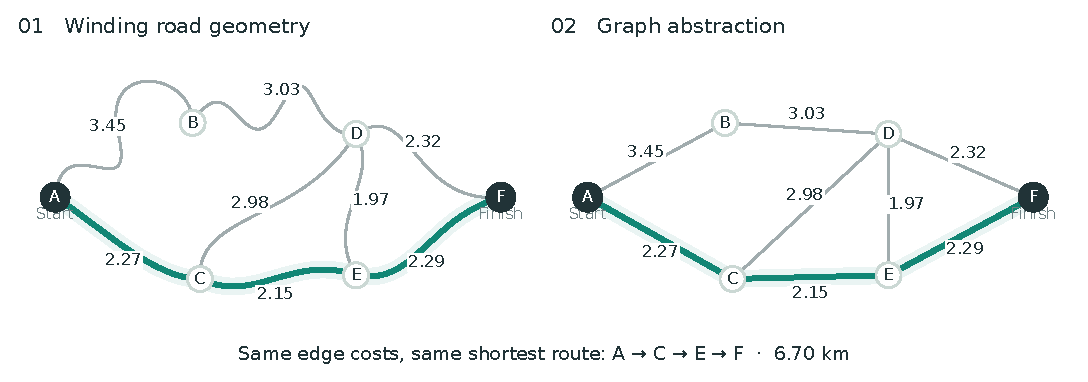
\includegraphics[width=.98\linewidth]{road_network.pdf}
\caption{Road geometry and its straight-edge abstraction retain the same
arc-length costs in illustrative kilometers and the same $6.70$ km
shortest route. The junctions are a separate example from the lattice experiments.}
\label{fig:roads}
\end{figure}

A road curve $\gamma_e:[0,1]\to\R^2$ has arc length
\[
 w(e)=\int_0^1\|\gamma_e'(t)\|_2\,dt.
\]
Endpoints are vertices; curves represent travel costs between discrete
junctions \cite{landers}. Straightening the drawing while retaining these
costs preserves all path costs and optima. In Figure~\ref{fig:roads},
arc lengths select $A\to C\to E\to F$; replacing weights by chord lengths
selects $A\to B\to D\to F$.

Lengths are approximated with 600 line segments per cubic Bezier piece.
Doubling this resolution agrees within relative tolerance $10^{-5}$.
Optimization uses unrounded values; labels show rounded costs.

\section{Reproducible structural experiment}
\paragraph{Design.}
We measure edges, triangles, and candidate distance evaluations on an
$s\times s$ lattice of spacing $1.2$, with independent coordinate jitter
in $[-0.07,0.07]$ and NumPy seed 2026. Distinct sites differ in some
coordinate by at least $1.06$ after jitter, certifying $k=1$.
The growth sweep uses $s=8,12,20,32,48$ at $R/k=1.7$; the range sweep
fixes $s=28$ and uses seven radii from $1.01$ to $5$. Increasing $s$
expands the region; changing $R$ preserves the points. Measurements
describe this family and seed.

\begin{table}[tbp]
\centering\small
\begin{tabular}{rrrrr}
\toprule
$n$ & Edges & Triangles & Grid distance checks & All pairs\\
\midrule
64 & 165 & 106 & 396 & 2,016\\
144 & 397 & 266 & 996 & 10,296\\
400 & 1,137 & 754 & 2,936 & 79,800\\
1,024 & 2,951 & 1,934 & 8,044 & 523,776\\
2,304 & 6,747 & 4,470 & 18,294 & 2,653,056\\
\bottomrule
\end{tabular}
\caption{Counts at $k=1$, $R=1.7$. Grid checks are candidate distance evaluations.}
\label{tab:experiment}
\end{table}

\begin{figure}[tbp]
\centering
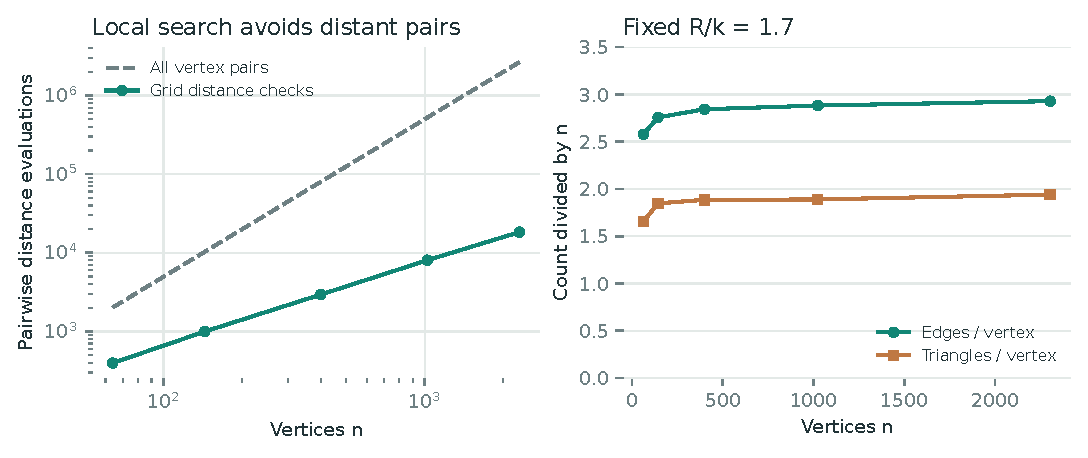
\includegraphics[width=\linewidth]{network_growth.pdf}
\caption{Fixed $R/k=1.7$: local distance checks versus all pairs (left),
and bounded edge and triangle counts per vertex (right). Lines join measured instances.}
\label{fig:growth}
\end{figure}

\paragraph{Results.}
At $n=2{,}304$, construction checks $18{,}294$ candidate distances against
$2{,}653{,}056$ all-pairs distances: about $145$ times fewer evaluations.
Running time also includes cell probes, hashing, loops, and storage.
The graph has $6{,}747$ edges and $4{,}470$ triangles, with bounded counts
per vertex across the growth sweep (Figure~\ref{fig:growth}). Larger
$R/k$ increases degree and triangles per vertex (Figure~\ref{fig:range});
at $R/k=1.01$, all vertices are isolated. The area bound stays above the
observed maximum degree.

\begin{figure}[tbp]
\centering
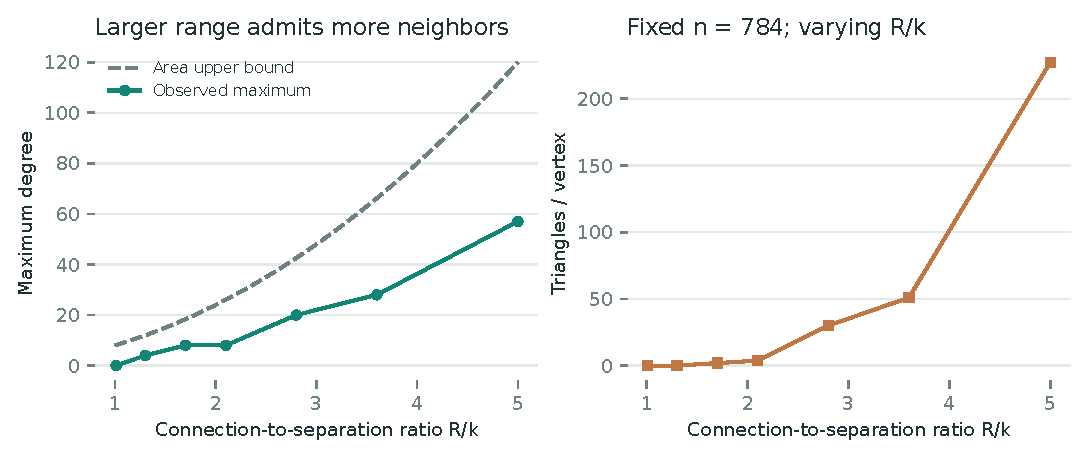
\includegraphics[width=\linewidth]{range_sensitivity.pdf}
\caption{Varying $R/k$ on $784$ fixed vertices: maximum degree and its
bound $(1+2R/k)^2-1$ (left), and graph triangles per vertex (right).}
\label{fig:range}
\end{figure}

\paragraph{Independent checks.}
The 80 grouped checks compare adjacency and triangles with exhaustive
enumeration and Dijkstra distances with SciPy Floyd--Warshall. They cover
the stated bounds, cutoff equality, negative cell coordinates,
disconnected graphs, empty and singleton inputs, and road arc lengths,
chord-weight route changes, and refinement agreement.

\paragraph{Arithmetic and reproducibility.}
Proofs assume exact real arithmetic and constant-cost floor operations;
the code uses IEEE floating-point coordinates and direct comparisons.
Near cutoffs or cell boundaries, robust predicates or higher precision
may be appropriate, with costs charged accordingly. Reproduce from the root:
\begin{verbatim}
python -m graph_traversal.experiment
python -m graph_traversal.validate
python -m graph_traversal.figures
\end{verbatim}
Inputs are generated locally; raw counts, environment metadata, code, and
vector figures are included. Build the paper with two \texttt{pdflatex}
runs from its directory.

\section{Related work}
This paper gives a self-contained specialization of disjoint-ball packing,
spatial hashing, and standard graph algorithms to minimum separation and
locality. Cabello and Jej\v{c}i\v{c} \cite{cabello} obtain $O(n\log n)$
single-source paths in unweighted unit-disk graphs using their geometric
representation, including dense instances. Here the assumptions bound
explicit adjacency size and allow supplied curved-road costs.

The project's one-stop note \cite{onestop} sorts feasibility thresholds
and stores prefix optima for logarithmic cutoff queries with one
intermediate stop. The triangle companion \cite{triangles} quantifies
shape exclusion under specified sampling laws. Local occupancy connects
the minimum-distance premise to graph density and traversal costs here.

\paragraph{Conclusion.}
Separation $k$ bounds local occupancy; connection radius $R$ turns it
into a degree bound. Fixed dimension and $R/k$ yield linear edge and
triangle counts, expected linear-time radius-graph construction, and
standard sparse-graph traversal bounds. The ratio $R/k$ controls these costs.

\begin{thebibliography}{9}
\small
\setlength{\itemsep}{2pt}
\bibitem{dijkstra}
E. W. Dijkstra, A note on two problems in connexion with graphs,
\emph{Numerische Mathematik} \textbf{1} (1959), 269--271.
\href{https://doi.org/10.1007/BF01386390}{doi:10.1007/BF01386390}.

\bibitem{chiba}
N. Chiba and T. Nishizeki, Arboricity and subgraph listing algorithms,
\emph{SIAM Journal on Computing} \textbf{14}(1) (1985), 210--223.
\href{https://doi.org/10.1137/0214017}{doi:10.1137/0214017}.

\bibitem{cabello}
S. Cabello and M. Jej\v{c}i\v{c}, Shortest paths in intersection graphs
of unit disks, \emph{Computational Geometry} \textbf{48}(4) (2015),
360--367.
\href{https://doi.org/10.1016/j.comgeo.2014.12.003}{doi:10.1016/j.comgeo.2014.12.003}.

\bibitem{landers}
J. R. Landers, \emph{Consequences of Minimum Distance in Mathematics
and Physics}, project manuscript (2026),
\href{https://github.com/jonland82/minimum-distance-analytical-mechanics/blob/master/consequences_of_minimum_distance.tex}{source}.

\bibitem{onestop}
J. R. Landers, \emph{One-stop routing with a changing distance cutoff},
project note (2026),
\href{https://github.com/jonland82/minimum-distance-analytical-mechanics/blob/master/routing_note/one_stop_routing.tex}{source}.

\bibitem{triangles}
J. R. Landers, \emph{How large must a triangle be to survive? Minimum-distance
exclusion under two sampling laws}, project note (2026),
\href{https://github.com/jonland82/minimum-distance-analytical-mechanics/blob/master/triangle_companion/triangle_exclusion.tex}{source}.
\end{thebibliography}
\end{document}
